%%%%%%%%%%%%%%%%%%%%%%%%%%%%%%%%%%%%%%%%%%%%%%%%%%%%%%%%%%%%
% 电磁学笔记
% 作者: Smeraldo
% 日期: 2025.3.17
%%%%%%%%%%%%%%%%%%%%%%%%%%%%%%%%%%%%%%%%%%%%%%%%%%%%%%%%%%%%

\documentclass[12pt, UTF8, AutoFakeBold]{ctexart} % 文章文档类,12pt 字号

% ========== 基本包 ==========
\usepackage{amsmath, amssymb, amsthm, esint} % 数学符号、定理环境
\usepackage{geometry} % 控制页面布局
\geometry{a4paper, margin=1in} % 设置 A4 纸张,1 英寸边距
\usepackage{subfigure}
\usepackage{graphicx} % 插入图片
\usepackage{xcolor} % 颜色支持
\usepackage{tcolorbox} % 重点内容高亮
\usepackage{hyperref} % 超链接支持
\hypersetup{
    colorlinks=true,
    linkcolor=blue,
    urlcolor=magenta
}

% ========== 定理、定义、引理 ==========
% \newtheorem{theorem}{定理}[section]
% \newtheorem{definition}{定义}[section]
% \newtheorem{lemma}{引理}[section]
\newtheorem{example}{例}[section]

% ========== 常用数学符号定义 ==========
\newcommand{\R}{\mathbb{R}} % 实数集
\newcommand{\dx}{\,dx} % 微分符号
\newcommand{\limn}{\lim_{n\to\infty}} % 极限格式

% ========== 目录 ==========
\begin{document}

\tableofcontents % 生成目录
\clearpage

\section{柱坐标系和球坐标系}

\subsection{柱坐标系}
柱坐标系相当于把直角坐标系中的$x$、$y$换为二维极坐标$\rho$、$\varphi$,同时保留z轴.柱坐标变量
$u_1 = \rho$、$u_2 = \varphi$、$u_3 = z$与直角坐标变量$x$、$y$、$z$的变换关系如下:
\[
    \begin{cases}
        x = \rho \cos\varphi\\
        y = \rho \sin\varphi\\
        z = z
    \end{cases}
    \text{或}
    \begin{cases}
        \rho = \sqrt{x^2 + y^2}\\
        \tan\varphi =  \frac{y}{x}\\
        z = z
    \end{cases}
\]
柱坐标系三个变量的范围:
\[
    0 \leq \rho < +\infty, \quad
    0 \leq \varphi < 2\pi, \quad
    -\infty < z < +\infty
\]

\begin{figure}[htbp]
    \centering
    \subfigure[柱坐标系]{
        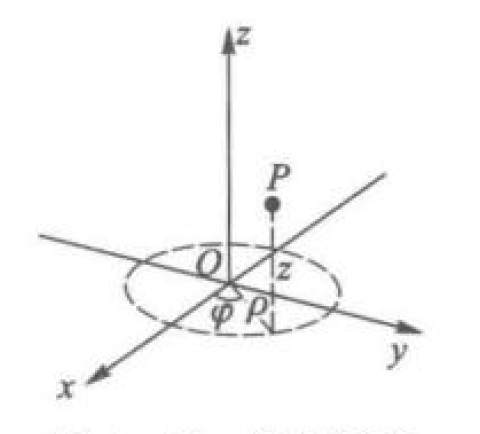
\includegraphics[width=0.25\textwidth]{images/柱坐标系.png}
    }
    \qquad
    \subfigure[柱坐标系的面元与体积元]{
        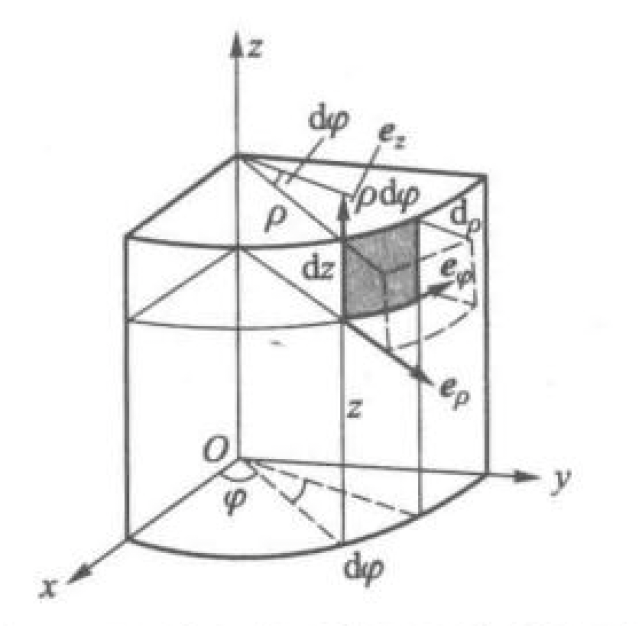
\includegraphics[width=0.25\textwidth]{images/柱坐标系的面元与体积元.png}
    }
\end{figure}

\subsection{球坐标系}
球坐标系的三个坐标变量是矢径的长度$r$、径矢与$z$轴的夹角$\theta$,和径矢在$xy$平面上的投影与$x$轴的夹角
$\varphi$.球坐标变量比$u_1 = r,u_2 = \theta,u_3 = \varphi$与直角坐标变量$x,y,z$的变换关系如下:
\[
    \begin{cases}
        x = r \sin\theta \cos\varphi\\
        y = r \sin\theta \sin\varphi\\
        z = r \cos\theta
    \end{cases}
    \text{或}
    \begin{cases}
        r = \sqrt{x^2 + y^2 + z^2}\\
        \cos\theta = \frac{z}{\sqrt{x^2 + y^2 + z^2}}\\
        \tan\varphi = \frac{y}{x}
    \end{cases}
\]
球坐标系三个变量的范围:
\[
    0 \leq r < +\infty, \quad
    0 \leq \theta \leq \pi, \quad
    0 \leq \varphi < 2\pi
\]

\begin{figure}[htbp]
    \centering
    \subfigure[球坐标系]{
        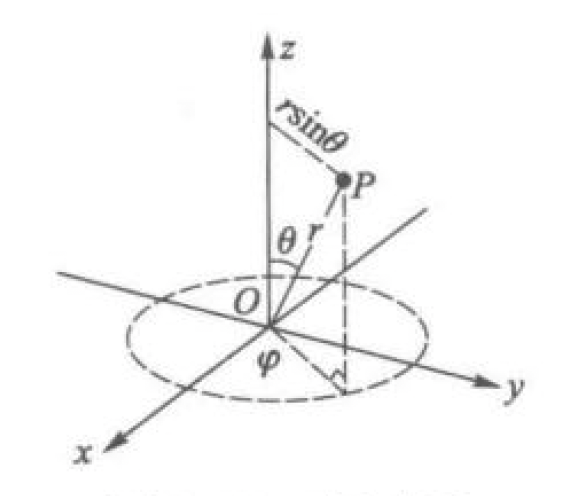
\includegraphics[width=0.25\textwidth]{images/球坐标系.png}
    }
    \qquad
    \subfigure[球坐标系的面元与体积元]{
        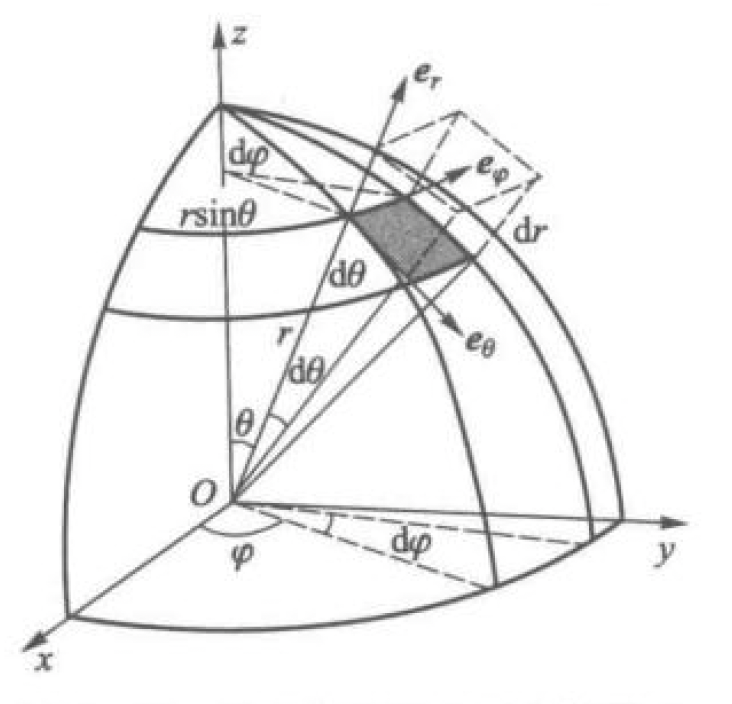
\includegraphics[width=0.25\textwidth]{images/球坐标系的面元与体积元.png}
    }
\end{figure}


\section{矢量分析提要}

\subsection{哈密顿算子或称耐普拉算子}
直角坐标
\[
    \nabla = \frac{\partial}{\partial x}\vec{i}
    + \frac{\partial}{\partial y}\vec{j}
    + \frac{\partial}{\partial z}\vec{k}
\]

柱坐标
\[
    \nabla = \frac{\partial}{\partial \rho}\vec{e_\rho}
    + \frac{1}{\rho} \frac{\partial}{\partial\varphi}\vec{e_\varphi}
    + \frac{\partial}{\partial z}\vec{e_z}
\]

球坐标
\[
    \nabla = \frac{\partial}{\partial r}\vec{e_r}
    + \frac{1}{r} \frac{\partial}{\partial \theta}\vec{e_\theta}
    + \frac{1}{r \sin\theta} \frac{\partial}{\partial \varphi}\vec{e_\varphi}
\]

算符$\nabla\cdot\nabla$常写作$\nabla^2$,叫作拉普拉斯算符.

\bigskip
\noindent 推导过程

柱坐标
\allowdisplaybreaks
\begin{align*}
    \because
    \vec{e_\rho} &= \cos\varphi\,\vec{i} + \sin\varphi\,\vec{j}\\
    \vec{e_\varphi} &= -\sin\varphi\,\vec{i} + \cos\varphi\,\vec{j}\\
    \therefore
    \begin{pmatrix}
        \vec{e_\rho}\\
        \vec{e_\varphi}\\
        \vec{e_z}
    \end{pmatrix}
    &=
    \begin{pmatrix}
        \cos\varphi & \sin\varphi & 0\\
        -\sin\varphi & \cos\varphi & 0\\
        0 & 0 & 1
    \end{pmatrix}
    \begin{pmatrix}
        \vec{i}\\
        \vec{j}\\
        \vec{k}
    \end{pmatrix}\\
    \begin{pmatrix}
        \vec{i}\\
        \vec{j}\\
        \vec{k}
    \end{pmatrix}
    &=
    \begin{pmatrix}
        \cos\varphi & -\sin\varphi & 0\\
        \sin\varphi & \cos\varphi & 0\\
        0 & 0 & 1
    \end{pmatrix}
    \begin{pmatrix}
        \vec{e_\rho}\\
        \vec{e_\varphi}\\
        \vec{e_z}
    \end{pmatrix}\\
    \text{又}\because
    \frac{\partial}{\partial\rho} &= \frac{\partial x}{\partial\rho}\frac{\partial}{\partial x}
    + \frac{\partial y}{\partial\rho}\frac{\partial}{\partial y}
    + \frac{\partial z}{\partial\rho}\frac{\partial}{\partial z}\\
    &= \cos\varphi\frac{\partial}{\partial x} + \sin\varphi\frac{\partial}{\partial y}\\
    \frac{\partial}{\partial\varphi} &= \frac{\partial x}{\partial\varphi}\frac{\partial}{\partial x}
    + \frac{\partial y}{\partial\varphi}\frac{\partial}{\partial y}
    + \frac{\partial z}{\partial\varphi}\frac{\partial}{\partial z}\\
    &= -\rho\sin\varphi\frac{\partial}{\partial x} + \rho\sin\varphi\frac{\partial}{\partial y}\\
    \therefore
    \begin{pmatrix}
        \frac{\partial}{\partial\rho}\\
        \frac{\partial}{\partial\varphi}\\
        \frac{\partial}{\partial z}
    \end{pmatrix}
    &=
    \begin{pmatrix}
        \cos\varphi & \sin\varphi & 0\\
        -\rho\sin\varphi & \rho\cos\varphi & 0\\
        0 & 0 & 1
    \end{pmatrix}
    \begin{pmatrix}
        \frac{\partial}{\partial x}\\
        \frac{\partial}{\partial y}\\
        \frac{\partial}{\partial z}
    \end{pmatrix}\\
    \begin{pmatrix}
        \frac{\partial}{\partial x}\\
        \frac{\partial}{\partial y}\\
        \frac{\partial}{\partial z}
    \end{pmatrix}
    &=
    \begin{pmatrix}
        \cos\varphi & -\frac{1}{\rho}\sin\varphi & 0\\
        \sin\varphi & \frac{1}{\rho}\cos\varphi & 0\\
        0 & 0 & 1
    \end{pmatrix}
    \begin{pmatrix}
        \frac{\partial}{\partial\rho}\\
        \frac{\partial}{\partial\varphi}\\
        \frac{\partial}{\partial z}
    \end{pmatrix}
\end{align*}
\begin{gather*}
    \therefore
    \nabla = \left(\cos\varphi\frac{\partial}{\partial\rho}
    - \frac{1}{\rho}\sin\varphi\frac{\partial}{\partial\varphi}\right)
    \left(\cos\varphi\vec{e_\rho} - \sin\varphi\vec{e_\varphi}\right)\\
    + \left(\sin\varphi\frac{\partial}{\partial\rho}
    + \frac{1}{\rho}\cos\varphi\frac{\partial}{\partial\varphi}\right)
    \left(\sin\varphi\vec{e_\rho} + \cos\varphi\vec{e_\varphi}\right)
    + \frac{\partial}{\partial z}\vec{e_z}\\
    \hspace{-200pt}\text{化简得}\\
    \nabla = \frac{\partial}{\partial \rho}\vec{e_\rho}
    + \frac{1}{\rho} \frac{\partial}{\partial\varphi}\vec{e_\varphi}
    + \frac{\partial}{\partial z}\vec{e_z}
\end{gather*}

球坐标
\allowdisplaybreaks
\begin{align*}
    \because
    \vec{e_r} &= \sin\theta\cos\varphi\,\vec{i} + \sin\theta\sin\varphi\,\vec{j} + \cos\theta\,\vec{k}\\
    \vec{e_\varphi} &= -\sin\varphi\,\vec{i} + \cos\varphi\,\vec{j}\;(\vec{k}\text{分量为}0)\\
    \vec{e_\theta} &= \cos\theta\cos\varphi\,\vec{i} + \cos\theta\sin\varphi\,\vec{j} - \sin\theta\,\vec{k}\\
    \therefore
    \begin{pmatrix}
        \vec{e_r}\\
        \vec{e_\theta}\\
        \vec{e_\varphi}
    \end{pmatrix}
    &=
    \begin{pmatrix}
        \sin\theta\cos\varphi & \sin\theta\sin\varphi & \cos\theta\\
        \cos\theta\cos\varphi & \cos\theta\sin\varphi & -\sin\theta\\
        -\sin\varphi & \cos\varphi & 0
    \end{pmatrix}
    \begin{pmatrix}
        \vec{i}\\
        \vec{j}\\
        \vec{k}
    \end{pmatrix}\\
    \begin{pmatrix}
        \vec{i}\\
        \vec{j}\\
        \vec{k}
    \end{pmatrix}
    &=
    \begin{pmatrix}
        \sin\theta\cos\varphi & \cos\theta\cos\varphi & -\sin\varphi\\
        \sin\theta\sin\varphi & \cos\theta\sin\varphi & \cos\varphi\\
        \cos\theta & -\sin\theta & 0
    \end{pmatrix}
    \begin{pmatrix}
        \vec{e_r}\\
        \vec{e_\theta}\\
        \vec{e_\varphi}
    \end{pmatrix}\\
    \text{又}\because
    \frac{\partial}{\partial r} &= \frac{\partial x}{\partial r}\frac{\partial}{\partial x}
    + \frac{\partial y}{\partial r}\frac{\partial}{\partial y}
    + \frac{\partial z}{\partial r}\frac{\partial}{\partial z}\\
    &= \sin\theta\cos\varphi\frac{\partial}{\partial x}
    + \sin\theta\sin\varphi\frac{\partial}{\partial y}
    + \cos\theta\frac{\partial}{\partial z}\\
    \frac{\partial}{\partial\theta} &= \frac{\partial x}{\partial\theta}\frac{\partial}{\partial x}
    + \frac{\partial y}{\partial\theta}\frac{\partial}{\partial y}
    + \frac{\partial z}{\partial\theta}\frac{\partial}{\partial z}\\
    &= r\cos\theta\cos\varphi\frac{\partial}{\partial x}
    + r\cos\theta\sin\varphi\frac{\partial}{\partial y}
    - r\sin\theta\frac{\partial}{\partial z}\\
    \frac{\partial}{\partial\varphi} &= \frac{\partial x}{\partial\varphi}\frac{\partial}{\partial x}
    + \frac{\partial y}{\partial\varphi}\frac{\partial}{\partial y}
    + \frac{\partial z}{\partial\varphi}\frac{\partial}{\partial z}\\
    &= -r\sin\theta\sin\varphi\frac{\partial}{\partial x}
    + r\sin\theta\cos\varphi\frac{\partial}{\partial y}\\
    \therefore
    \begin{pmatrix}
        \frac{\partial}{\partial r}\\
        \frac{\partial}{\partial\theta}\\
        \frac{\partial}{\partial\varphi}
    \end{pmatrix}
    &=
    \begin{pmatrix}
        \sin\theta\cos\varphi & \sin\theta\sin\varphi & \cos\theta\\
        r\cos\theta\cos\varphi & r\cos\theta\sin\varphi & -r\sin\theta\\
        -r\sin\theta\sin\varphi & r\sin\theta\cos\varphi & 0
    \end{pmatrix}
    \begin{pmatrix}
        \frac{\partial}{\partial x}\\
        \frac{\partial}{\partial y}\\
        \frac{\partial}{\partial z}\\
    \end{pmatrix}\\
    \begin{pmatrix}
        \frac{\partial}{\partial x}\\
        \frac{\partial}{\partial y}\\
        \frac{\partial}{\partial z}\\
    \end{pmatrix}
    &=
    \begin{pmatrix}
        \sin\theta\cos\varphi & \frac{1}{r}\cos\theta\cos\varphi & -\frac{\sin\varphi}{r\sin\theta}\\
        \sin\theta\sin\varphi & \frac{1}{r}\cos\theta\sin\varphi & \frac{\cos\varphi}{r\sin\theta}\\
        \cos\theta & -\frac{1}{r}\sin\theta & 0
    \end{pmatrix}
    \begin{pmatrix}
        \frac{\partial}{\partial r}\\
        \frac{\partial}{\partial\theta}\\
        \frac{\partial}{\partial\varphi}
    \end{pmatrix}\\
\end{align*}
\begin{gather*}
    \therefore
    \nabla = \left(\sin\theta\cos\varphi\frac{\partial}{\partial r}
    + \frac{1}{r}\cos\theta\cos\varphi\frac{\partial}{\partial\theta}
    - \frac{\sin\varphi}{r\sin\theta}\frac{\partial}{\partial\varphi}\right)
    \left(\sin\theta\cos\varphi\vec{e_r}
    + \cos\theta\cos\varphi\vec{e_\theta}
    - \sin\varphi\vec{e_\varphi}\right)\\
    + \left(\sin\theta\sin\varphi\frac{\partial}{\partial r}
    + \frac{1}{r}\cos\theta\sin\varphi\frac{\partial}{\partial\theta}
    + \frac{\cos\varphi}{r\sin\theta}\frac{\partial}{\partial\varphi}\right)
    \left(\sin\theta\sin\varphi\vec{e_r}
    + \cos\theta\sin\varphi\vec{e_\theta}
    + \cos\varphi\vec{e_\varphi}\right)\\
    + \left(\cos\theta\frac{\partial}{\partial r}
    - \frac{1}{r}\sin\theta\frac{\partial}{\partial\theta}\right)
    \left(\cos\theta\vec{e_r} - \sin\theta\vec{e_\theta}\right)\\
    \hspace{-300pt}\text{化简得}\\
    \nabla = \frac{\partial}{\partial r}\vec{e_r}
    + \frac{1}{r} \frac{\partial}{\partial \theta}\vec{e_\theta}
    + \frac{1}{r \sin\theta} \frac{\partial}{\partial \varphi}\vec{e_\varphi}
\end{gather*}

\subsection{场}
标量场:空间各点存在着一个标量$\varphi$,它的数值是空间位置的函数.

矢量场:空间各点存在着一个矢量$\vec{E}$,它的大小和方向是空间位置的函数.

\subsection{标量场梯度}
\subsubsection{定义}
梯度:一个空间位置函数的的变化率.它沿方向微商最大的方向,数值上等于这个最大的方向微商
$\frac{\partial \varphi}{\partial n}$,其中沿$\Delta n$方向的方向微商为
\[
    \frac{\partial \varphi}{\partial n} = \lim_{\Delta n \to 0}\frac{\Delta \varphi}{\Delta n}
\]
$\Delta n$的方向是两等值面间最短的位移矢量.

\begin{figure}[htbp]
    \centering
    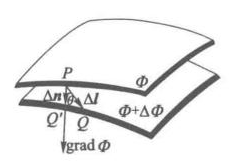
\includegraphics[width=0.25\textwidth]{images/标量场的梯度.png}
    \caption{标量场的梯度}
\end{figure}

梯度意义:空间某点标量场函数的最大变化率,刻画了标量场的空间分布特征.已知梯度即可求沿任一方向的方向导数.

\textbf{标量场的梯度是个矢量场.}
\subsubsection{坐标表示式}
直角坐标
\[
    \nabla\varPhi = \frac{\partial\varPhi}{\partial x}\vec{i}
    + \frac{\partial\varPhi}{\partial y}\vec{j}
    + \frac{\partial\varPhi}{\partial z}\vec{k}
\]

柱坐标
\[
    \nabla\varPhi = \frac{\partial\varPhi}{\partial\rho}\vec{e_\rho}
    + \frac{1}{\rho} \; \frac{\partial\varPhi}{\partial\varphi}\vec{e_\varphi}
    + \frac{\partial\varPhi}{\partial z}\vec{e_z}
\]

球坐标
\[
    \nabla\varPhi = \frac{\partial\varPhi}{\partial r}\vec{e_r}
    + \frac{1}{r} \; \frac{\partial\varPhi}{\partial\theta}\vec{e_\theta}
    + \frac{1}{r\sin\theta} \; \frac{\partial\varPhi}{\partial\varphi}\vec{e_\varphi}
\]

\subsection{矢量场通量和散度}
\subsubsection{定义}
通量:矢量场通过一个截面的面积分为通量
\[
    \varPhi_A = \iint_{S} \boldsymbol{A} \cdot d\boldsymbol{S} = \iint_S A\cos\theta dS
\]
式中$\theta$为$A$与面元$dS$的法线之间的夹角.

散度:令$S$为一闭合曲面,包含体积为$\Delta V$.当体积趋向于空间某点$P$,$\Delta V \to 0$,$\varPhi_A$也趋于零.
若两者之比有一极限,则这极限值为矢量场在$P$点的散度,记作$div \, \boldsymbol{A}$或$\nabla \cdot \boldsymbol{A}$.
\[
    \nabla \cdot \boldsymbol{A} = \lim_{\Delta V \to 0}\frac{\varPhi_A}{\Delta V} = 
    \lim_{\Delta V \to 0}\frac{\oiint_S\boldsymbol{A} \cdot d\boldsymbol{S}}{\Delta V}
\]

散度的意义:用来描述空间某一范围内场的发散或汇聚,具有局域性质.

\textbf{矢量场的散度是个标量场.}
\subsubsection{散度的坐标表示式}
直角坐标
\[
    \nabla \cdot \boldsymbol{A} = \frac{\partial A_x}{\partial x}
    + \frac{\partial A_y}{\partial y}
    + \frac{\partial A_z}{\partial z}
\]

柱坐标
\[
    \nabla \cdot \boldsymbol{A} = \frac{1}{\rho}\frac{\partial}{\partial\rho}(\rho A_\rho)
    + \frac{1}{\rho}\frac{\partial A_\varphi}{\partial\varphi}
    + \frac{\partial A_z}{\partial z}
\]

球坐标
\[
    \nabla \cdot \boldsymbol{A} =
    \frac{1}{r^2}\left[\frac{\partial}{\partial r}(r^2 A_r)\right]
    + \frac{1}{r\sin\theta}\left[\frac{\partial}{\partial\theta}(\sin\theta A_\theta)\right]
    + \frac{1}{r\sin\theta}\frac{\partial A_\varphi}{\partial\varphi}
\]

\subsection{矢量场的环量和旋度}
\subsubsection{定义}
环量:矢量场$\boldsymbol{A}$沿闭合回路$L$的线积分为环量
\[
    \varGamma_A = \oint_L\boldsymbol{A} \cdot d\boldsymbol{l}
\]

旋度:令$\Delta S$为一闭合曲线包围的面积。当回路缩小至空间某点$P$,$\Delta S \to 0$,$\varGamma_A$
也趋于零.若两者之比有一极限,则这极限值为矢量场在$P$点的旋度.$\boldsymbol{A}$的旋度记作
$curl \, \boldsymbol{A}$或$rot \, \boldsymbol{A}$,或$\nabla \times \boldsymbol{A}$.
\[
    (\nabla \times \boldsymbol{A})_n = \lim_{\Delta S \to 0}\frac{\Delta\varGamma_A}{\Delta S}
    = \lim_{\Delta S \to 0}\frac{\oint_L\boldsymbol{A} \cdot d\boldsymbol{l}}{\Delta S}
\]

旋度的意义:$\varGamma_A = 0$表明在区域内无涡旋状态,场线不闭合.$\varGamma_A \neq 0$表明在区域内存在涡旋状态,场线闭合.

\textbf{矢量场的旋度是个矢量场.}
\subsubsection{旋度的坐标表示式}
直角坐标
\begin{align*}
    \nabla \times \boldsymbol{A} &=
    \left(\frac{\partial A_z}{\partial y} - \frac{\partial A_y}{\partial z}\right)\vec{i}
    + \left(\frac{\partial A_x}{\partial z} - \frac{\partial A_z}{\partial x}\right)\vec{j}
    + \left(\frac{\partial A_y}{\partial x} - \frac{\partial A_x}{\partial y}\right)\vec{k}\\
    &=
    \begin{vmatrix}
        \vec{i} & \vec{j} & \vec{k}\\
        \frac{\partial}{\partial x} & \frac{\partial}{\partial y} & \frac{\partial}{\partial z}\\
        A_x & A_y & A_z
    \end{vmatrix}
\end{align*}

柱坐标
\begin{align*}
    \nabla \times \boldsymbol{A} &=
    \left(\frac{1}{\rho}\frac{\partial A_z}{\partial \varphi} - \frac{\partial A_\varphi}{\partial z}\right)\vec{e_\rho}
    + \left(\frac{\partial A_\rho}{\partial z} - \frac{\partial A_z}{\partial \rho}\right)\vec{e_\varphi}
    + \frac{1}{\rho}\left(\frac{\partial(\rho A_\varphi)}{\partial \rho} - \frac{\partial A_\rho}{\partial \varphi}\right)\vec{e_z}\\
    &=
    \begin{vmatrix}
        \vec{e_\rho} & \vec{e_\varphi} & \vec{e_z}\\
        \frac{\partial}{\partial \rho} & \frac{1}{\rho} \frac{\partial}{\partial \varphi} & \frac{\partial}{\partial z}\\
        A_\rho & A_\varphi & A_z
    \end{vmatrix}
\end{align*}

球坐标
\begin{align*}
    \nabla \times \boldsymbol{A} &=
    \left[\frac{1}{r\sin\theta}\left(\frac{\partial}{\partial\theta}(A_\varphi \sin\theta) - \frac{\partial A_\theta}{\partial\varphi}\right)\right]\vec{e_r}
    + \left[\frac{1}{r} \, \frac{1}{\sin\theta} \, \frac{\partial A_r}{\partial \varphi} - \frac{1}{r}\left(\frac{\partial}{\partial r}(r A_\varphi)\right)\right]\vec{e_\theta}\\
    &+ \left[\frac{1}{r} \, \frac{\partial (r A_\theta)}{\partial r} - \frac{1}{r} \, \frac{\partial A_r}{\partial\theta}\right]\vec{e_\varphi}\\
    &=
    \begin{vmatrix}
        \vec{e_r} & \vec{e_\theta} & \vec{e_\varphi}\\
        \frac{\partial}{\partial r} & \frac{1}{r} \frac{\partial}{\partial\theta} & \frac{1}{r \sin\theta}\frac{\partial}{\partial\varphi}\\
        A_r & A_\theta & A_\varphi
    \end{vmatrix}
\end{align*}

\subsection{矢量的定理}
高斯定理:矢量场通过任意闭合曲面$S$的通量等于它包含的体积$V$内的散度的积分
\[
    \oiint_S\boldsymbol{A} \cdot d\boldsymbol{S} = \iiint_V \nabla \cdot \boldsymbol{A}dV
\]

斯托克斯定理:矢量场在任意闭合回路$L$上的环量等于以它为边界的曲面$S$上旋度的积分
\[
    \oint_L\boldsymbol{A} \cdot d\boldsymbol{l} = \iint_S (\nabla \times \boldsymbol{A}) \cdot d\boldsymbol{S}
\]

\subsection{一些定理}
\vspace{-2.5em}
\begin{gather*}
    \nabla(fg) = f(\nabla g) + (\nabla f)g\\
    \nabla \times (\nabla f) = 0\\
    \nabla \cdot (\,\nabla \times \vec{f}\,) = 0\\
    \nabla \times (\,\nabla \times \vec{f}\,) = \nabla (\,\nabla \cdot \vec{f}\,) - \nabla^2 \vec{f}
\end{gather*}

\section{静电场}

\subsection{库仑定律}
适用于两个点电荷相互作用
\[
    \vec{F}_{12}=k\frac{q_1q_2}{r_{12}^2}\hat{r}_{12}
\]

SI制:$k=\frac{1}{4\pi\varepsilon_0},\vec{F}_{12}=\frac{1}{4\pi\varepsilon_0}\frac{q_1q_2}{r_{12}^2}\hat{r}_{12}$

$\varepsilon_0$真空介电常数:$\varepsilon_0=8.854187817\times 10^{-12}\;C^2/(N\cdot m^2)$

库仑(C)的定义:由电流单位安培(A)导出 , 1C=1A$\cdot$s

\subsection{电场强度}
\subsubsection{电场强度}
静电场中任一点处的电场强度,等于单位正电荷在该点处所受的电场力。(含大小和方向)

SI制单位:N/C,或 V/m

点电荷q的场强:
\[
    \vec{E}=\frac{1}{4\pi\varepsilon_0}\frac{q}{r^2}\hat{r}
\]
\subsubsection{场强叠加原理}
点荷系$q_1,q_2,\dots,q_n$或$q_i(i=1,2,\dots,n)$

$q_0$受力
\[
    \vec{F}=\vec{f}_1+\vec{f}_2+\dots+\vec{f}_n=\sum\limits_{i=1}^{n}\vec{f}_i,
\]

其中$\vec{f}_i=\frac{q_0q_i}{4\pi\varepsilon_0r_i^2}\hat{r_i}$

除以$q_0$:
\[
    \frac{\vec{F}}{q_0}=\sum\limits_{i=1}^{n}\frac{\vec{f_i}}{q_0}=
    \frac{1}{4\pi\varepsilon_0}\sum\limits_{i=1}^{n}\frac{q_i}{r_i^3}\vec{r_i}
\]

可写成
\begin{gather*}
    \vec{E}=\sum\limits_{i=1}^{n}\vec{E_i}\\
    \text{或}\vec{E}=\frac{1}{4\pi\varepsilon_0}\int_{q}\frac{dq}{r^3}\vec{r}
\end{gather*}
\subsubsection{场强的计算}
依据:1)场强的定义;2)库仑定律;3)场强叠加原理。

点电荷的场:
\[
    \vec{E}=\frac{q\vec{r}}{4\pi\varepsilon_0 r^3}
\]

电荷系的场:
\[
    \vec{E}=\frac{1}{4\pi\varepsilon_0}\sum\limits_{i=1}^{n}\frac{q_i}{r_i^3}\vec{r_i}
\]

连续带电体的场:
\[
    \vec{E}=\frac{1}{4\pi\varepsilon_0}\int_{q}\frac{dq}{r^3}\vec{r}
\]
\begin{example}[电偶极子]
    两点电荷$+q$和$-q$,相距l,$\vec{l}$的方向由$-q$指向$+q$,当考察点至两电荷的距离$r\gg l$时,
    两点电荷可视为一电荷对,称为电偶极子。

    定义电偶极矩:$\vec{p}=q\vec{l}$(简称电矩),$\vec{l}$是极轴(从负电荷指向正电荷的矢径);电矩的值$p_e=ql$\\
    求电偶极子的场强($r\gg l$)

    $1$)场点P在$\vec{l}$的延长线上
    \begin{gather*}
        E_+=\frac{q}{4\pi\varepsilon_0(r-\frac{l}{2})^2},\;
        E_-=\frac{q}{4\pi\varepsilon_0(r+\frac{l}{2})^2}\\
        \hspace{-300pt}\text{则总场强}\\
        E_1=\frac{q}{4\pi\varepsilon_0}\left[\frac{1}{(r-\frac{l}{2})^2}-
        \frac{1}{(r+\frac{l}{2})^2}\right]
        =\frac{q}{4\pi\varepsilon_0}\frac{2rl}{\left[r^2-\left(\frac{l}{2}\right)^2\right]^2}\\
        \hspace{-200pt}\text{因}r\gg l\text{则}r^2-\left(\frac{l}{2}\right)^2\approx r^2\\
        \hspace{-326pt}\text{故}\\
        E_1=\frac{1}{4\pi\varepsilon_0}\frac{2ql}{r^3}
        \;\text{或}\;
        E_1=\frac{1}{4\pi\varepsilon_0}\frac{2\vec{p}}{r^3}
    \end{gather*}

    $2$)场点P在$\vec{l}$的中垂线上
    \begin{gather*}
        E_+=E_-=\frac{q}{4\pi\varepsilon_0}\frac{1}{r^2+\left(\frac{l}{2}\right)^2}\\
        \hspace{-300pt}\text{则总场强}\\
        E_2=2E_+\cos\alpha\\
        \hspace{-300pt}\text{而}\\
        \cos\alpha=\frac{\frac{l}{2}}{\sqrt{r^2+\left(\frac{l}{2}\right)^2}}\\
        \hspace{-300pt}\text{得}\\
        E_2=\frac{q}{4\pi\varepsilon_0}\frac{l}{\left[r^2+\left(\frac{l}{2}\right)^2\right]^\frac{3}{2}}\\
        \hspace{-200pt}\text{因}r\gg l\text{则}r^2+\left(\frac{l}{2}\right)^2\approx r^2\\
        \hspace{-326pt}\text{故}\\
        E_2=\frac{ql}{4\pi\varepsilon_0r^3}
        \;\text{或}\;
        E_2=\frac{1}{4\pi\varepsilon_0}\frac{-\vec{p}}{r^3}
    \end{gather*}

    \begin{figure}[htbp]
        \centering
        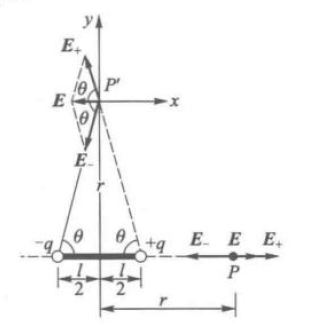
\includegraphics[width=0.25\textwidth]{images/电偶极子的场强.png}
        \caption{电偶极子的场强}
    \end{figure}

    $3$)场点P在远处任一位置
    \begin{gather*}
        E_+=\frac{q}{4\pi\varepsilon_0r_+^2},\;E_-=\frac{q}{4\pi\varepsilon_0r_-^2}\\
        \hspace{-140pt}\text{将$\vec{E_+},\vec{E_-}$分别沿着$\vec{r}$和垂直于$\vec{r}$方向分解}\\
        \begin{aligned}
            E_r&=E_+\cos(\theta_1-\theta)-E_-\cos(\theta-\theta_2)\\
            &\approx E_+-E_-=\frac{q}{4\pi\varepsilon_0}(\frac{1}{r_+^2}-\frac{1}{r_-^2})\\
            &=\frac{q}{4\pi\varepsilon_0}\frac{(r_-+r_+)(r_--r_+)}{r_+^2\cdot r_-^2}\\
            &\approx\frac{q}{4\pi\varepsilon_0}\frac{2rl\cos\theta}{r^4}\\
            &=\frac{2\cos\theta}{4\pi\varepsilon_0 r^3}p_e
        \end{aligned}\\
        \begin{aligned}
            E_\theta&=E_+\sin(\theta_1-\theta)-E_-\sin(\theta-\theta_2)\\
            &=\frac{q}{4\pi\varepsilon_0r_+^2r_-^2}\left[r_-^2\sin(\theta_1-\theta)+r_+^2\sin(\theta-\theta_2)\right]\\
            &=\frac{ql\sin\theta}{2\times 4\pi\varepsilon_0r_+^2r_-^2}\left(r_++r_-\right)\\
            &=\frac{\sin\theta}{4\pi\varepsilon_0 r^3}p_e
        \end{aligned}\\
        \hspace{-300pt}\text{场强的大小:}\\
        E_3=\sqrt{E_r^2+E_\theta^2}=\frac{p_e}{4\pi\varepsilon_0 r^3}\sqrt{3\cos^2\theta+1}\\
        \hspace{-300pt}\text{场强的方向:}\\
        \tan\alpha=\frac{E_\theta}{E_r}=\frac{1}{2}\tan\theta,\\
        \hspace{-238pt}\text{其中$\alpha$为$\vec{E_3}$与$\vec{r}$的夹角}\\
    \end{gather*}
\end{example}

\end{document}
